\documentclass[a4paper,10pt]{article}
\usepackage[utf8]{inputenc}
\usepackage{graphicx}
\usepackage{float}
\usepackage{hyperref}

%opening
\title{GPGPU Prac 2: The Mandelbrot Set}
\author{Antonio Peters}

\begin{document}

\maketitle

\section{The Mandelbrot Set}
The Mandelbrot Set is a collection of complex numbers $c$ such that iterating the equation
\begin{equation}
  z_{i+1} = z_i^2 + c, \qquad z_0=0
\end{equation}
does not tend to infinity.
\linebreak
For this to hold true, firstly the number must be within radius $2$ of the origin, $0$. The set generated can be seen in Figure \ref{mandelimg}
\begin{figure}[H] \label{mandelimg}
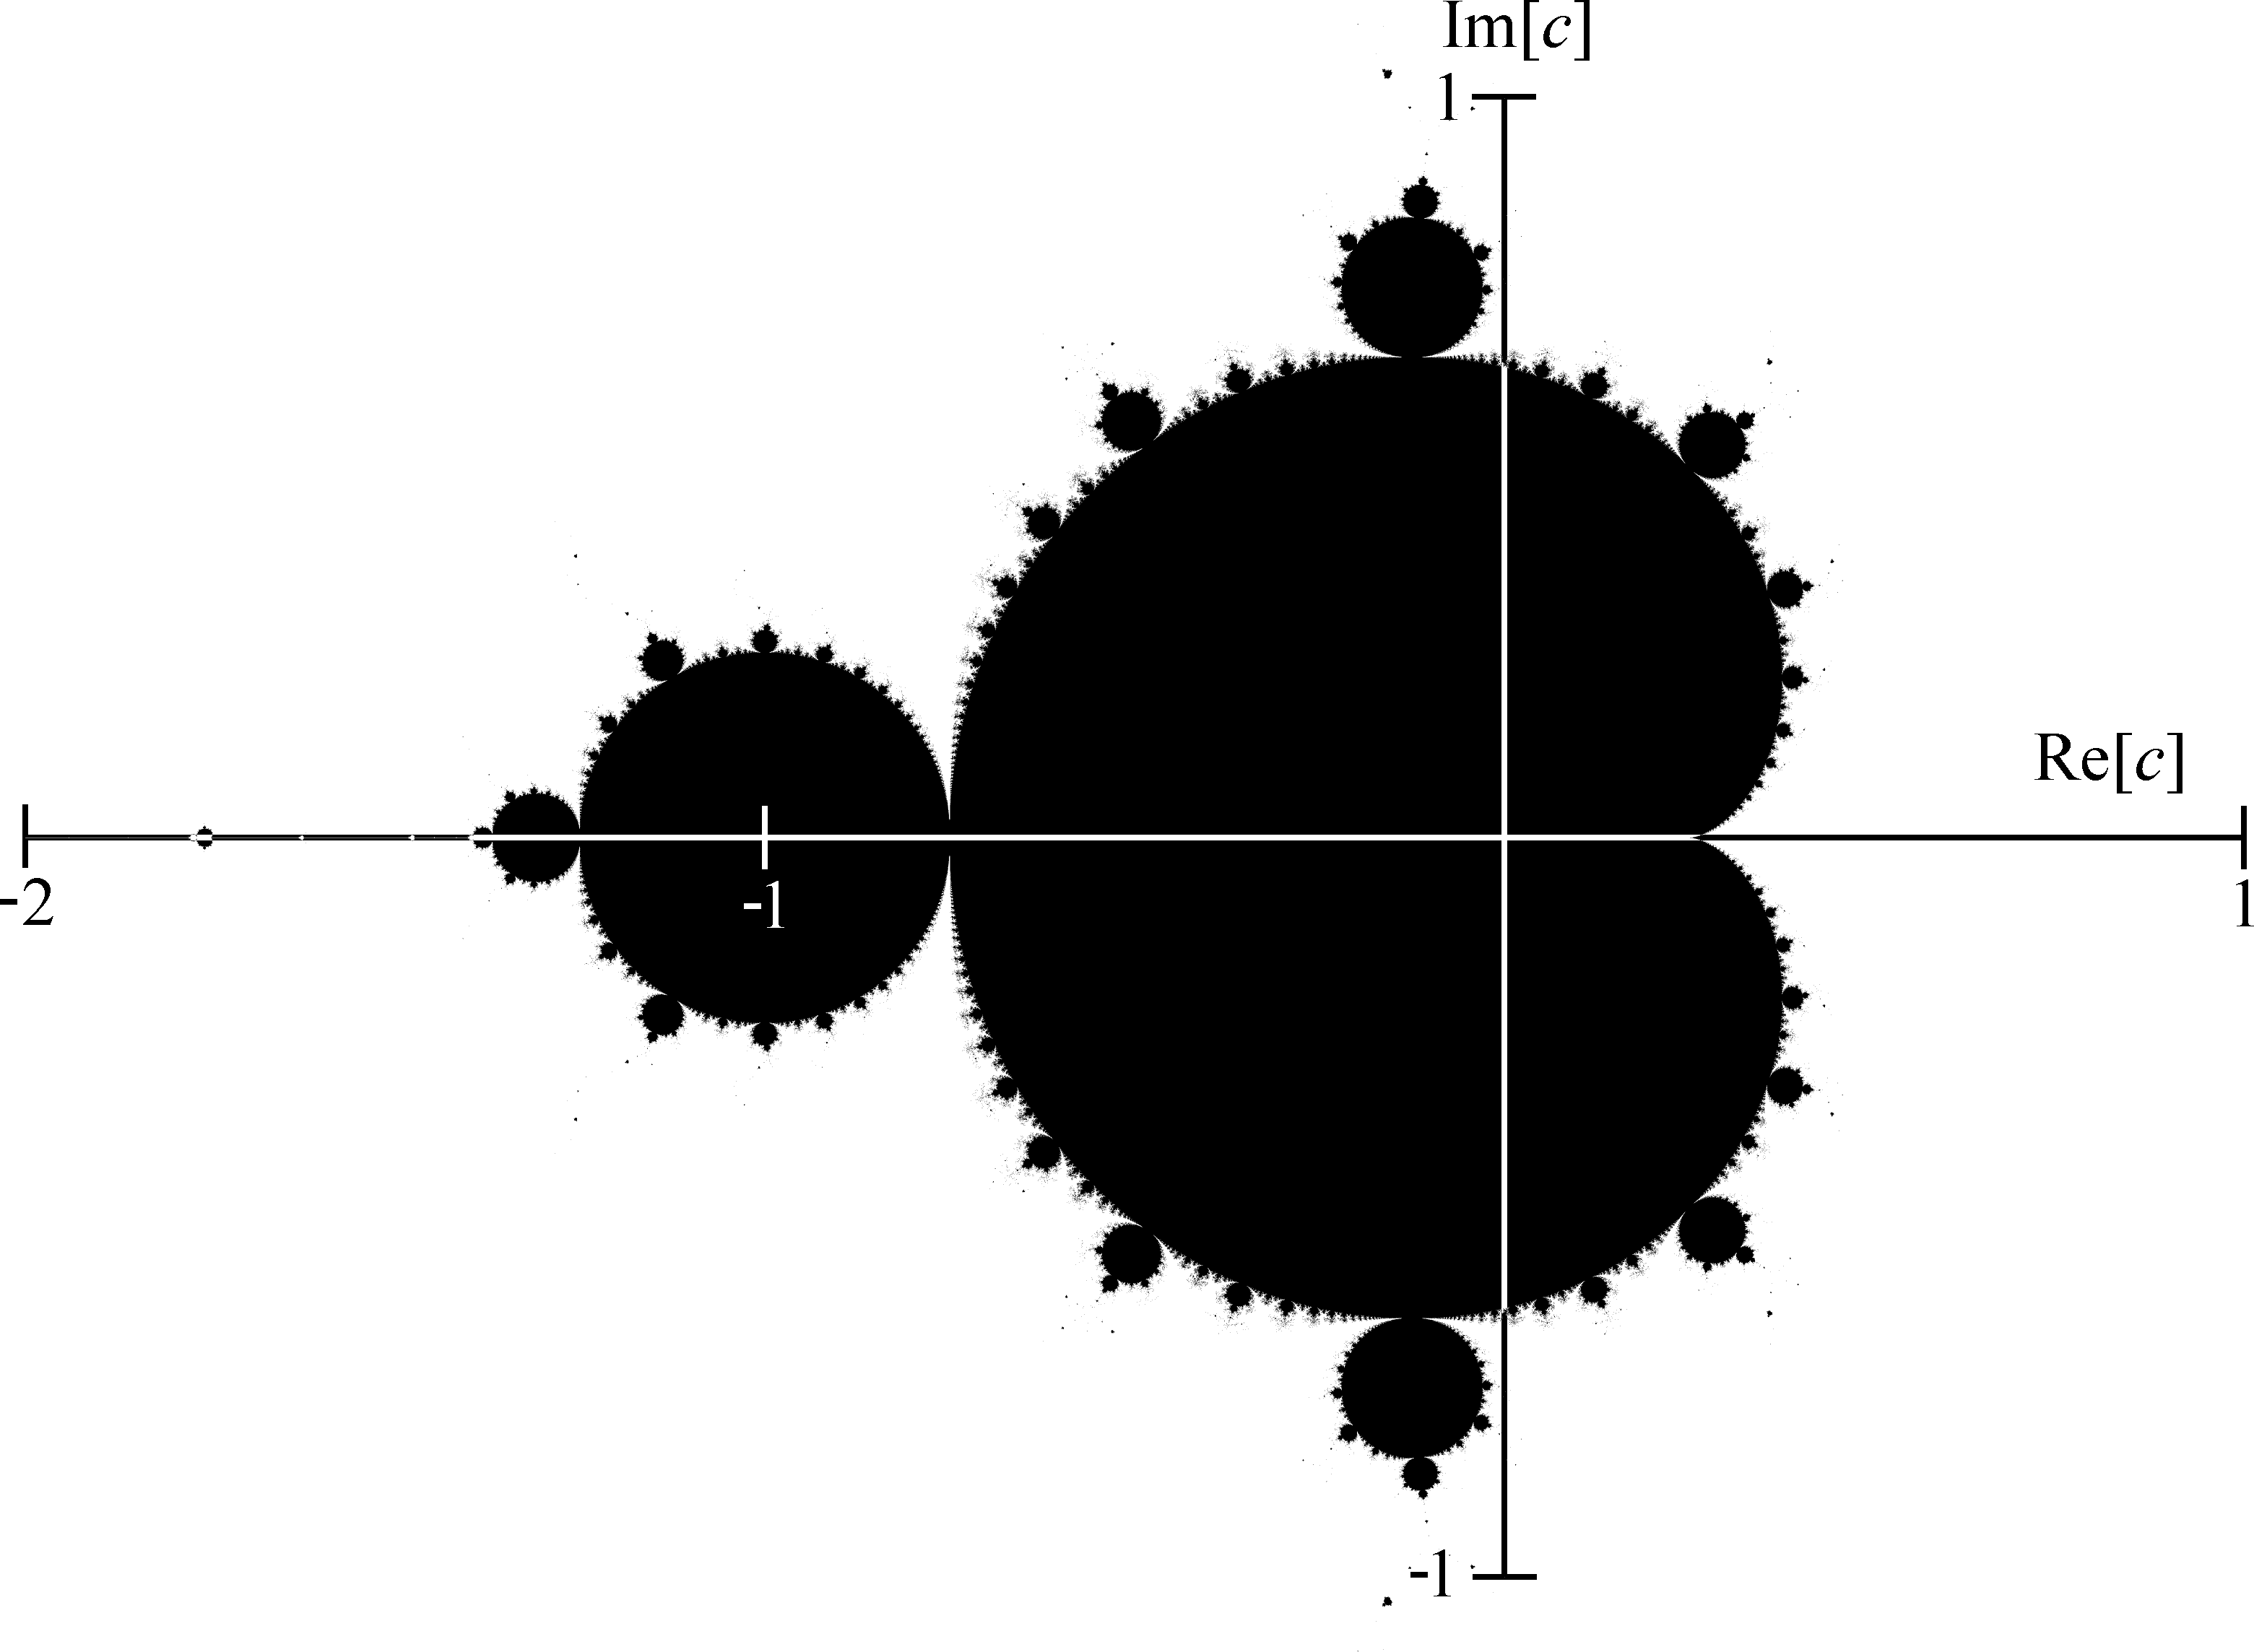
\includegraphics[width=\textwidth]{Mandelset_hires.png}
\caption{The Mandelbrot Set}
\end{figure}
The most interesting notion about this is the fact that the pattern generated by the Mandelbrot Set is recursive, each node on the surface of the main lobe has on its surface a replicate set of nodes and similarly for these subnodes extending infinitely. In order to study this however we need to reduce this amount, we do this by setting the size of the image being generated and setting an upper limit to the number of iterations the set goes through. In the case of this task these particular settings were set to $4096$x$4096$ for the image size and $10000$ for the maximum number of iterations.

\section{CPU Implementation}
The code used to generate a CPU implementation of the Mandelbrot Set was originally taken from \url{https://rosettacode.org/wiki/Mandelbrot_set#C}, the code was then re-factored to be better ported to a GPU such that the only differences between them were the essential elements being timed. The code works by nesting two for-loops and iterating over the X- and Y-axis and calculating the whether or not the point, scaled to fit on the $(-2,-2i) to (2,2i)$ plane, is in the Mandelbrot Set for the given number of iterations. This linear method generated the set in $115453.000000$ milliseconds, setting a baseline for the GPU implementation to work on.

\section{Naive GPU Implementation}
The GPU implementation was created by taking the general algorithm of the CPU implementation and assigning a thread to each point of the set, further divided into blocks and grids. Since the the 10000 iterations for set inclusion rely on each other, this could not be parallelized. Once calculated, the data is then transferred back to the CPU, to be written to a file in the exact same manner as the CPU implementation to minimize the differences between them to only that of the actual algorithm implementation. The time taken by this method is $5341.878418$ milliseconds, a fraction of the time of that of the CPU time. However, further analysis through the NVIDIA Visual Profiler shows that this too can be improved on. Although the process uses $100\%$ of its computation capacity, it does not use any computation/memory transfer capabilities to overlap data transfers.

\section{Optimized GPU Implementation}
Due to the nature of the Mandelbrot Set code, no data is read in to be used, it simply takes generates an x,y-coordinate using the threads data and then scales it before computing the point so there are no reads which need optimizing and there is only one transfer of data, namely from the GPU to the CPU, so this is the only way in which memory can be optimized. Therefore, streams were introduced to allow for asynchronous data transfers. Using two streams an execution time of $5335.469727$ milliseconds, a very minor speed up, but it also alludes to the fact that with larger data sets, the overhead cost of having streams can be made up for with the ability to asynchronously transfer data.
\linebreak
\linebreak
Although compute occupancy could not be increased, an approach with fewer threads was looked at with data iterations in the kernel, meaning each thread calculates more than one point value. This was tested with two calculations per thread for a time of $5309.734863$, again only a minor speed up given that the data set is large with an unparallizable loop of $10000$ iterations but it is the only way to increase the computational optimization of the program.
\linebreak
\linebreak
Since there is only one kernel and no kernel memory reads, there is no possibility for latency optimization other that the streams, which have already been explored.
\linebreak
\linebreak
By utilizing both streams, asynchronous data transfers, and multiple iterations per thread we get a compounded speed up with an execution time of $5273.914551$, which is faster than either of the optimizations on their own.

\end{document}
